%-----BEGIN DISCLAIMER-----
%******************************************************************************
% Copyright (c) 2011, 2021 JCrypTool Team and Contributors
%
% All rights reserved. This program and the accompanying materials
% are made available under the terms of the Eclipse Public License v1.0
% which accompanies this distribution, and is available at
% http://www.eclipse.org/legal/epl-v10.html
%******************************************************************************
%-----END DISCLAIMER-----

% This is a redraw of an old pixel graphic in svg vector format for the
% online help of the JCrypTool plug-in "Simple Power Analysis".
%
% To build the svg, you require: 
%
%  * a LaTeX distribution (https://latex-project.org/)
%  * the TikZ/PGF package (https://ctan.org/pkg/pgf)
%  * ImageMagick's convert on path (https://imagemagick.org/)
%
% If requirements are fulfilled, run following command (--shell-escape is important):
% pdflatex --shell-escape secure-sam-power-graph.tex
% 
% ADJUST THE LANGUAGE by setting the macro "\imagelanguage" to german or english below
\documentclass[tikz,convert=pdf2svg]{standalone}
\usepackage{pgfplots}
\usepackage{ifthen}
\usetikzlibrary{calc, positioning,decorations.pathreplacing}
\pgfplotsset{compat=1.17}

%*********************************************
% Adjust the language here (german or english)
%*********************************************
%\newcommand{\imagelanguage}{german}
\newcommand{\imagelanguage}{english}

\begin{document}
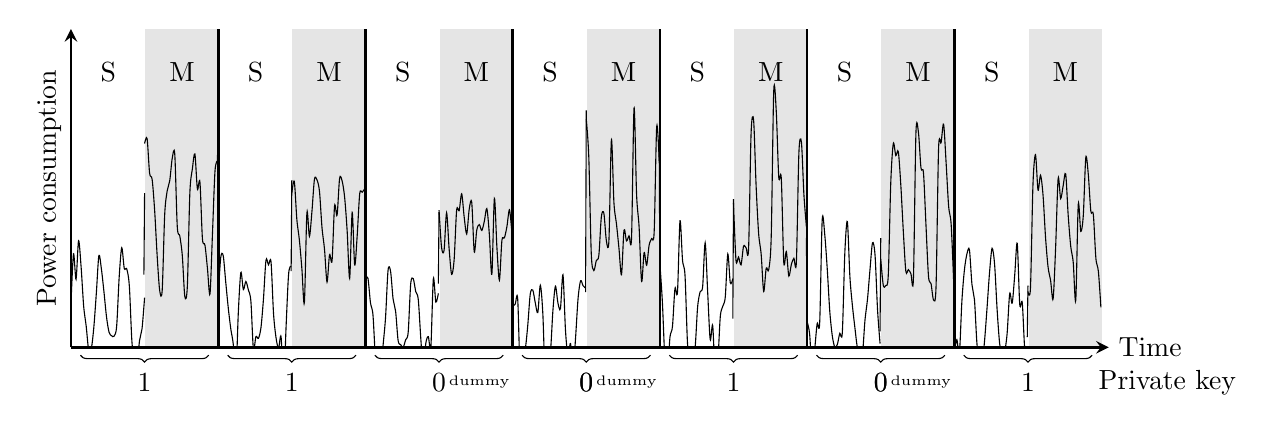
\begin{tikzpicture}[declare function={
      excitation(\t,\w) = sin(\t*\w);
      noise = rnd - 0.5;
      source(\t,\o) = excitation(\t,10) + noise + \o;
      filter(\t) = 1 - abs(sin(mod(\t, 35)));
      speech(\t,\o) = 1 + source(\t,\o)*filter(\t);
    }
  ]
  \pgfmathsetmacro{\D}{110}
  \pgfmathsetmacro{\scale}{2.6}
  \pgfmathsetmacro{\scalesmall}{0.6}
  \pgfmathsetmacro{\bdist}{0.12pt}



\ifthenelse{\equal{\imagelanguage}{german}}%
%True
{
  \pgfmathsetmacro{\ylabel}{"Energieverbrauch"}
  \pgfmathsetmacro{\xlabel}{"Zeit"}
  \pgfmathsetmacro{\key}{"Privater Schlüssel"}
  \pgfmathsetmacro{\keyoffset}{10}

}
%False
{
  \pgfmathsetmacro{\ylabel}{"Power consumption"}
  \pgfmathsetmacro{\xlabel}{"Time"}
  \pgfmathsetmacro{\key}{"Private key"}
  \pgfmathsetmacro{\keyoffset}{16}
}

  \pgfplotsset{ticks=none}
  \begin{axis}[
    width=420,
    height=160,
    axis on top=true,
    axis lines = middle,
    axis line style={line width=1pt},
    y label style={at={(axis description cs:0, 0.5)},rotate=90,anchor=south},
    x label style={at={(axis description cs:1, 0)}, anchor=west},
    restrict x to domain*=0:2000,
    restrict y to domain*=0:10,
    xlabel={\xlabel},
    ylabel={\ylabel},
    xmin=0,
    xmax=1100,
    ymin=2.2,
    ymax=2.6,
    axis background/.style={%
      preaction={
        path picture={
          \node[fill=gray!20, minimum width=\D*0.0085cm, minimum height=7cm, anchor=west] at (\D*0.0085cm, 1cm) {};
          \node[fill=gray!20, minimum width=\D*0.0085cm, minimum height=7cm, anchor=west] at (\D*3*0.0085cm, 1cm) {};
          \node[fill=gray!20, minimum width=\D*0.0085cm, minimum height=7cm, anchor=west] at (\D*5*0.0085cm, 1cm) {};
          \node[fill=gray!20, minimum width=\D*0.0085cm, minimum height=7cm, anchor=west] at (\D*7*0.0085cm, 1cm) {};
          \node[fill=gray!20, minimum width=\D*0.0085cm, minimum height=7cm, anchor=west] at (\D*9*0.0085cm, 1cm) {};
          \node[fill=gray!20, minimum width=\D*0.0085cm, minimum height=7cm, anchor=west] at (\D*11*0.0085cm, 1cm) {};
          \node[fill=gray!20, minimum width=\D*0.0085cm, minimum height=7cm, anchor=west] at (\D*13*0.0085cm, 1cm) {};
    }}}]
  ]


    %% Main lines
    \draw[black, x=0.0085cm, y=0.8cm, yshift=-20pt] plot [domain=0:\D, samples=30, smooth] (\x,{speech(\x, \scalesmall)});
    \draw[black, x=0.0085cm, y=0.8cm, yshift=-20pt] plot [domain=\D:\D*2-1, samples=30, smooth] (\x,{speech(\x, \scale)});
    \draw[black, x=0.0085cm, y=0.8cm, yshift=-20pt] plot [domain=\D*2:\D*3-1, samples=30, smooth] (\x,{speech(\x, \scalesmall)});
    \draw[black, x=0.0085cm, y=0.8cm, yshift=-20pt] plot [domain=\D*3:\D*4-1, samples=30, smooth] (\x,{speech(\x, \scale)});
    \draw[black, x=0.0085cm, y=0.8cm, yshift=-20pt] plot [domain=\D*4:\D*5-1, samples=30, smooth] (\x,{speech(\x, \scalesmall)});
    \draw[black, x=0.0085cm, y=0.8cm, yshift=-20pt] plot [domain=\D*5:\D*6-1, samples=30, smooth] (\x,{speech(\x, \scale)});
    \draw[black, x=0.0085cm, y=0.8cm, yshift=-20pt] plot [domain=\D*6:\D*7-1, samples=30, smooth] (\x,{speech(\x, \scalesmall)});
    \draw[black, x=0.0085cm, y=0.8cm, yshift=-20pt] plot [domain=\D*7:\D*8-1, samples=30, smooth] (\x,{speech(\x, \scale)});
    \draw[black, x=0.0085cm, y=0.8cm, yshift=-20pt] plot [domain=\D*8:\D*9-1, samples=30, smooth] (\x,{speech(\x, \scalesmall)});
    \draw[black, x=0.0085cm, y=0.8cm, yshift=-20pt] plot [domain=\D*9:\D*10-1, samples=30, smooth] (\x,{speech(\x, \scale)});
    \draw[black, x=0.0085cm, y=0.8cm, yshift=-20pt] plot [domain=\D*10:\D*11-1, samples=30, smooth] (\x,{speech(\x, \scalesmall)});
    \draw[black, x=0.0085cm, y=0.8cm, yshift=-20pt] plot [domain=\D*11:\D*12-1, samples=30, smooth] (\x,{speech(\x, \scale)});
    \draw[black, x=0.0085cm, y=0.8cm, yshift=-20pt] plot [domain=\D*12:\D*13-1, samples=30, smooth] (\x,{speech(\x, \scalesmall)});
    \draw[black, x=0.0085cm, y=0.8cm, yshift=-20pt] plot [domain=\D*13:\D*14-1, samples=30, smooth] (\x,{speech(\x, \scale)});

    %% Connections
    \draw[black, x=0.0085cm, y=0.8cm, yshift=-20pt] ({(\D-1)*0.0085cm}, {speech(\D-1, \scalesmall)} ) -- ({\D*0.0085cm}, {speech(\D, \scale)});
    \draw[black, x=0.0085cm, y=0.8cm, yshift=-20pt] ({(\D*2-1)*0.0085cm}, {speech(\D*2-1, \scale)}) -- ({\D*2*0.0085cm}, {speech(\D*2, \scalesmall)});
    \draw[black, x=0.0085cm, y=0.8cm, yshift=-20pt] ({(\D*3-1)*0.0085cm}, {speech(\D*3-1, \scalesmall)}) -- ({\D*3*0.0085cm}, {speech(\D*3, \scale)});
    \draw[black, x=0.0085cm, y=0.8cm, yshift=-20pt] ({(\D*4-1)*0.0085cm}, {speech(\D*4-1, \scale)}) -- ({\D*4*0.0085cm}, {speech(\D*4, \scalesmall)});
    \draw[black, x=0.0085cm, y=0.8cm, yshift=-20pt] ({(\D*5-1)*0.0085cm}, {speech(\D*5-1, \scalesmall)}) -- ({\D*5*0.0085cm}, {speech(\D*5, \scale)});
    \draw[black, x=0.0085cm, y=0.8cm, yshift=-20pt] ({(\D*6-1)*0.0085cm}, {speech(\D*6-1, \scale)}) -- ({\D*6*0.0085cm}, {speech(\D*6, \scalesmall)});
    \draw[black, x=0.0085cm, y=0.8cm, yshift=-20pt] ({(\D*7-1)*0.0085cm}, {speech(\D*7-1, \scalesmall)}) -- ({\D*7*0.0085cm}, {speech(\D*7, \scale)});
    \draw[black, x=0.0085cm, y=0.8cm, yshift=-20pt] ({(\D*8-1)*0.0085cm}, {speech(\D*8-1, \scale)}) -- ({\D*8*0.0085cm}, {speech(\D*8, \scalesmall)});
    \draw[black, x=0.0085cm, y=0.8cm, yshift=-20pt] ({(\D*9-1)*0.0085cm}, {speech(\D*9-1, \scalesmall)}) -- ({\D*9*0.0085cm}, {speech(\D*9, \scale)});
    \draw[black, x=0.0085cm, y=0.8cm, yshift=-20pt] ({(\D*10-1)*0.0085cm}, {speech(\D*10-1, \scale)}) -- ({\D*10*0.0085cm}, {speech(\D*10, \scalesmall)});
    \draw[black, x=0.0085cm, y=0.8cm, yshift=-20pt] ({(\D*11-1)*0.0085cm}, {speech(\D*11-1, \scalesmall)}) -- ({\D*11*0.0085cm}, {speech(\D*11, \scale)});
    \draw[black, x=0.0085cm, y=0.8cm, yshift=-20pt] ({(\D*12-1)*0.0085cm}, {speech(\D*12-1, \scale)}) -- ({\D*12*0.0085cm}, {speech(\D*12, \scalesmall)});
    \draw[black, x=0.0085cm, y=0.8cm, yshift=-20pt] ({(\D*13-1)*0.0085cm}, {speech(\D*13-1, \scalesmall)}) -- ({\D*13*0.0085cm}, {speech(\D*13, \scale)});

    %% vertical fat lines (separating a loop in square-and-multiply)
    \draw[black, x=0.0085cm, y=0.8cm, yshift=-20pt, line width=1pt] ({(\D*2)*0.0085cm}, 0) -- ({\D*2*0.0085cm}, 10);
    \draw[black, x=0.0085cm, y=0.8cm, yshift=-20pt, line width=1pt] ({(\D*4)*0.0085cm}, 0) -- ({\D*4*0.0085cm}, 10);
    \draw[black, x=0.0085cm, y=0.8cm, yshift=-20pt, line width=1pt] ({(\D*6)*0.0085cm}, 0) -- ({\D*6*0.0085cm}, 10);
    \draw[black, x=0.0085cm, y=0.8cm, yshift=-20pt, line width=1pt] ({(\D*8)*0.0085cm}, 0) -- ({\D*8*0.0085cm}, 10);
    \draw[black, x=0.0085cm, y=0.8cm, yshift=-20pt, line width=1pt] ({(\D*10)*0.0085cm}, 0) -- ({\D*10*0.0085cm}, 10);
    \draw[black, x=0.0085cm, y=0.8cm, yshift=-20pt, line width=1pt] ({(\D*12)*0.0085cm}, 0) -- ({\D*12*0.0085cm}, 10);
  \end{axis}

  \draw[anchor=west, decorate, decoration = {brace} ] (\D*2*0.0085cm-\bdist cm, -0.1cm) -- (0 + \bdist cm, -0.1cm) node[below=3pt, midway] {1};
  \draw[anchor=west, decorate, decoration = {brace} ] (\D*4*0.0085cm-\bdist cm, -0.1cm) -- (\D*2*0.0085cm + \bdist cm, -0.1cm) node[below=3pt, midway] {1};
  \draw[anchor=west, decorate, decoration = {brace} ] (\D*6*0.0085cm-\bdist cm, -0.1cm) -- (\D*4*0.0085cm + \bdist cm, -0.1cm)
    node[below=3pt, midway] (number-4) {0} node[right=-6pt of number-4.east, anchor=west] () {\tiny dummy};
  \draw[anchor=west, decorate, decoration = {brace} ] (\D*8*0.0085cm-\bdist cm, -0.1cm) -- (\D*6*0.0085cm + \bdist cm, -0.1cm) node[below=3pt, midway] {0}
    node[below=3pt, midway] (number-6) {0} node[right=-6pt of number-6.east, anchor=west] () {\tiny dummy};
  \draw[anchor=west, decorate, decoration = {brace} ] (\D*10*0.0085cm-\bdist cm, -0.1cm) -- (\D*8*0.0085cm + \bdist cm, -0.1cm) node[below=3pt, midway] {1};
  \draw[anchor=west, decorate, decoration = {brace} ] (\D*12*0.0085cm-\bdist cm, -0.1cm) -- (\D*10*0.0085cm + \bdist cm, -0.1cm) node[below=3pt, midway] {0}
    node[below=3pt, midway] (number-10) {0} node[right=-6pt of number-10.east, anchor=west] () {\tiny dummy};
  \draw[anchor=west, decorate, decoration = {brace} ] (\D*14*0.0085cm-\bdist cm, -0.1cm) -- (\D*12*0.0085cm + \bdist cm, -0.1cm) node[below=3pt, midway] (last-anchor) {1};

  \node[right=\keyoffset pt of last-anchor.east] () {\key};


  \node[minimum width=\D*0.0085cm, anchor=west] at (0, 3.5cm) {S};
  \node[minimum width=\D*0.0085cm, anchor=west] at (\D*1*0.0085cm, 3.5cm) {M};
  \node[minimum width=\D*0.0085cm, anchor=west] at (\D*2*0.0085cm, 3.5cm) {S};
  \node[minimum width=\D*0.0085cm, anchor=west] at (\D*3*0.0085cm, 3.5cm) {M};
  \node[minimum width=\D*0.0085cm, anchor=west] at (\D*4*0.0085cm, 3.5cm) {S};
  \node[minimum width=\D*0.0085cm, anchor=west] at (\D*5*0.0085cm, 3.5cm) {M};
  \node[minimum width=\D*0.0085cm, anchor=west] at (\D*6*0.0085cm, 3.5cm) {S};
  \node[minimum width=\D*0.0085cm, anchor=west] at (\D*7*0.0085cm, 3.5cm) {M};
  \node[minimum width=\D*0.0085cm, anchor=west] at (\D*8*0.0085cm, 3.5cm) {S};
  \node[minimum width=\D*0.0085cm, anchor=west] at (\D*9*0.0085cm, 3.5cm) {M};
  \node[minimum width=\D*0.0085cm, anchor=west] at (\D*10*0.0085cm, 3.5cm) {S};
  \node[minimum width=\D*0.0085cm, anchor=west] at (\D*11*0.0085cm, 3.5cm) {M};
  \node[minimum width=\D*0.0085cm, anchor=west] at (\D*12*0.0085cm, 3.5cm) {S};
  \node[minimum width=\D*0.0085cm, anchor=west] at (\D*13*0.0085cm, 3.5cm) {M};
  \end{tikzpicture}
\end{document}
